\documentclass{article} % For LaTeX2e
\usepackage[utf8]{inputenc}
\usepackage{nips15submit_e,times}
\usepackage{hyperref}
\usepackage{graphicx}
\usepackage{subfigure}
\usepackage{hyperref}
\usepackage{url}
\usepackage{times}
\usepackage{epsfig}
\usepackage{graphicx}
\usepackage{amsmath}
\usepackage{amssymb}
\usepackage{multirow}
\usepackage{caption} 
\usepackage{url}
%\documentstyle[nips14submit_09,times,art10]{article} % For LaTeX 2.09

\title{Recurrent Batch Normalization}

\author{
Me \\
\And
Nicolas \\
\And
C\'esar \\
\And
Aaron
\texttt{email} \\
}

\newcommand{\fix}{\marginpar{FIX}}
\newcommand{\new}{\marginpar{NEW}}

%\nipsfinalcopy % Uncomment for camera-ready version

\usepackage{amsfonts}
\usepackage{amsmath}

\newcommand{\vect}[1]{\mathbf{#1}}
\newcommand{\mat}[1]{\mathbf{#1}}
\newcommand{\act}{f}
\newcommand{\ewprod}{\odot}
\newcommand{\reals}{\mathbb{R}}
\newcommand{\given}{\vert}

\bibliographystyle{plain}

\begin{document}

\maketitle

\begin{abstract}
We propose a reparameterization of LSTM that brings the benefits of batch normalization to recurrent neural networks.
Empirical results show faster convergence and improved generalization on classification, language modeling and speech transcription tasks.
\end{abstract}

\section{Introduction}


%% FIXME redo intro

%% Training deep neural networks by gradient descent is hard due in large part to pathological curvature in the objective function.
%% Approaches to alleviating this problem divide naturally into two categories: smarter optimization algorithms such as
%% Hessian-Free~\cite{hessianfree} and various approximations to natural gradient~\cite{amari} proposed in~\cite{ollivier} and~\cite{KFAC},
%% and model reparameterizations~\cite{efficientbackprop}~\cite{raiko}~\cite{naturalneuralnetworks}.

%Success of first order SGD depends on the  the curvature of the objective that is optimized~\cite{hessianfree} which depends on the networks parametrization~\cite{amari}.


%% It involves normalizing unit preactivations in order to make their distributions easier to control.
%% This greatly improves the training dynamics of deep feedforward neural networks, leading to faster convergence and better generalization.
%% Recently, a related technique called weight normalization~\cite{weightnorm} was introduced, which has a similar effect to batch normalization yet might be easier to carry over to the recurrent setting.
%% [also normprop]
%% However to our knowledge none of these schemes have yet been transferred to RNNs.



%%% This section mix up the argument of jacobian (backprop-through time) and hessian (high curvature) for hard optimization, need to be FIXED

Recurrent neural network architectures such as LSTM~\cite{lstm} and GRU~\cite{cho2014learning} have recently exhibited
state-of-the-art performance on a wide range of complex sequential problems including speech recognition~\cite{baidu},
machine translation~\cite{bahdanau2014neural} and image and video captioning~\cite{xu2015show,yao2015describing}.
Top-performing models, however, are based on very high-capacity networks that are computationally intensive and costly to train.
Effective optimization of recurrent neural networks is an active area of study.

It is known that for deep feed-forward neural networks, covariate shift~\cite{shimodaira2000improving,batchnorm}
degrades the efficiency of training.
Covariate shift is a change in distribution of the inputs to a model.
This occurs continuously during training of feed-forward neural networks,
where changing the parameters of a layer affects the distribution of the inputs to all layers above it.
As a result, the upper layers are continually adapting to the shifting input distribution and unable to learn effectively.
Covariate shift may play an especially important role in recurrent neural networks,
which resemble very deep feed-forward networks.

Batch normalization~\cite{batchnorm} is a recently proposed technique for controlling the distributions of feed-forward neural network activations, thereby reducing internal covariate shift.
It involves standardizing the activations going into each layer, enforcing their means and variances to be invariant to changes in the parameters of the underlying layers.
% relying on the observation that a network converges faster when its inputs have zero mean, unit variance and are uncorrelated~\cite{efficientbackprop}.
This effectively decouples each layer's parameters from those of other layers, leading to a better-conditioned optimization problem.
Indeed, deep neural networks trained with batch normalization converge significantly faster and generalize better.

Although batch normalization has demonstrated significant training speed-ups and generalization benefits in feedforward networks,
it has proven difficult to apply in recurrent architectures~\cite{cesar,baidu}.
It has found limited use in stacked RNNs, where the normalization is applied ``vertically'', i.e. to the input of each RNN, but not ``horizontally'' between timesteps.
RNNs are deepest in the time direction, and as such batch normalization would be most beneficial when applied horizontally.
However, it has been hypothesized~\cite{cesar} that applying batch normalization in this way hurts training
because of exploding gradients due to repeated rescaling.

Our findings run counter to this hypothesis.
We show that it is possible and highly beneficial to apply batch normalization in the hidden-to-hidden transition of recurrent models.
In particular, we describe a reparameterization of LSTM that involves batch normalization
and demonstrate that doing so speeds up optimization and improves generalization.
In addition, we empirically analyze the gradient backpropagation and show that proper initialization
of the batch normalization parameters is crucial to avoiding gradient vanishing.

We evaluate our proposal on several sequential problems and show that our
LSTM reparameterization consistently outperforms the LSTM baseline across tasks,
in terms of both time to convergence and performance.
In particular, we achieve state-of-the-art performance on Sequential MNIST~\cite{le2015simple} and FIXME.

%% FIXME add section 4
Section~\ref{sec:prerequisites} introduces RNNs and batch normalization in detail.
In Section~\ref{sec:recurrent-batch-normalization} we discuss batch normalization in the recurrent setting.
We show in Section~\ref{sec:experiments} our evaluations of the proposed re-parameterization on a variety of tasks.

\section{Prerequisites}
\label{sec:prerequisites}


\subsection{LSTM}

Long Short-Term Memory (LSTM) networks are an instance of a more general class of recurrent neural networks (RNNs),
which we shall briefly review.
Given an input sequence
$\mat{X} = ( \vect{x}_1, \vect{x}_2, ... \vect{x}_T )$,
an RNN defines a sequence of hidden states $h_t$ according to
\begin{eqnarray}
  \mat{h}_t = \phi(\mat{W}_h \vect{h}_{t-1} + \mat{W}_x  \vect{x}_t + \vect{b}),
\end{eqnarray}
where $\mat{W}_h \in \reals^{d_h \times d_h}, \mat{W}_x \in \reals^{d_x \times d_h}, \vect{b} \in \reals^{d_h}$
and the initial state $\vect{h}_0 \in \reals^{d_h}$ % I've put this back because I believe we do need to say something about the initial state -- tim
are model parameters.
A popular choice for the activation function $\phi$ is $\tanh$.

RNNs are popular in sequence modeling because of their natural ability to process variable-length sequences.
Training RNNs using first-order stochastic gradient descent (SGD) however is notoriously difficult
due to the well-known problem of exploding/vanishing gradients~\cite{bengio1994learning,hochreiter1991untersuchungen,pascanudifficulty}.
Gradient vanishing occurs when states $h_t$ are not influenced by small changes in much earlier states $h_{\tau}$, $t \ll \tau$,
preventing learning of long-term dependencies in the input data.
While the long-term dependencies problem is unsolvable in absolute~\cite{bengio1994learning},
it has been demonstrated that different RNN re-parameterizations, such as the LSTM~\cite{lstm}, GRU~\cite{cho2014learning} or $i$/$u$-RNN~\cite{le2015simple,urnn}
can help mitigate the vanishing gradient problem.

In what follows, we focus on the LSTM architecture~\cite{lstm} with recurrent transition given by
\begin{eqnarray}
\left(\begin{array}{ccc}
\tilde{\vect{f}}_t \\
\tilde{\vect{i}}_t \\
\tilde{\vect{o}}_t \\
\tilde{\vect{g}}_t
\end{array}\right)
 &=&
 \mat{W}_h \vect{h}_{t-1} +
 \mat{W}_x \vect{x}_t +
 \vect{b}
 \\
\vect{c}_t &= &\sigma(\tilde{\vect{f}}_t) \ewprod \vect{c}_{t-1} +
\sigma(\tilde{\vect{i}}_t) \ewprod \tanh(\tilde{\vect{g}_t}) \\
\vect{h}_t &= &\sigma(\tilde{\vect{o}}_t) \ewprod \tanh(\vect{c}_t),
\end{eqnarray}
where $\vect{W}_h \in \reals^{d_h \times 4 d_h}, \vect{W}_x \reals^{d_x \times 4 d_h}, \vect{b} \in \reals^{4 d_h}$
and the initial states $\vect{h}_0 \in \reals^{d_h}, \vect{c}_0 \in \reals^{d_h}$ % I've put this back because I believe we do need to say something about the initial state -- tim
are model parameters.
$\sigma$ is the logistic function, and the $\ewprod$ operator denotes the Hadamard product.

The LSTM differs from simple RNNs in that it has an additional memory \emph{cell} $\vect{c}_t$ whose update is nearly linear which allows the gradient to flow back through time more easily.
In addition, unlike the RNN which overwrites its content at each time-step,
the update of the LSTM cell is regulated by a set of gates.
The forget gate $\vect{f}_t$ determines the extent to which information is carried over from the previous time-step,
and the input gate $\vect{i}_t$ controls the flow of information from the current input $\vect{x}_t$.
The output gate $\vect{o}_t$ allows the model to read from the cell.
This carefully controlled interaction with the cell is what allows the LSTM to robustly retain information for long periods of time.

\subsection{Batch normalization}

\emph{Covariate shift}~\cite{shimodaira2000improving} is a phenomenon in machine learning where
the features presented to a model change in distribution during the course of training.
In order for learning to succeed in the presence of covariance shift,
the model's parameters must be adjusted not just to learn the concept at hand
but also to adapt to the changing distribution of the inputs.
In deep neural networks, this problem manifests as \emph{internal covariance shift}~\cite{batchnorm},
where changing the parameters of a layer affects the distribution of the inputs to all layers above it.

Batch Normalization~\cite{batchnorm} is a recently proposed network reparameterization that aims to reduce internal covariate shift.
It does so by standardizing the activations using statistical estimates of their means and standard deviations.
However, it does not decorrelate the activations as the matrix inversion involved would be too expensive.

The batch normalizing transform is as follows:

\begin{align}
\mathrm{BN}(\vect{h}; \gamma, \beta) =
  \beta + \gamma
  \frac{\vect{h} -   \widehat{\mathbb{E  }}(\vect{h})}
       {       \sqrt{\widehat{\mathrm{Var}}(\vect{h}) + \epsilon}}
\end{align}

where $\vect{h} \in \reals^d$ is the vector of (pre)activations to be normalized, $\gamma \in \reals^d, \beta \in \reals^d$ are model parameters that determine the mean and standard deviation of the normalized activation, and $\epsilon \in \reals$ is a regularization hyperparameter.
The division should be understood to proceed elementwise.

At training time, the statistics $\mathbb{E}(\vect{h})$ and $\mathrm{Var}(\vect{h})$ are estimated by the sample mean and sample variance of the current minibatch.
This allows for backpropagation through the statistics, preserving the convergence properties of stochastic gradient descent.
During inference, the statistics are typically estimated based on the entire training set, so as to produce a deterministic prediction.


\section{Batch-Normalized LSTM}
\label{sec:recurrent-batch-normalization}

This section introduces a reparameterization of LSTM that takes advantage of batch normalization.
Contrary to previous work~\cite{cesar, baidu}, we leverage batch normalization in both the input-to-hidden \emph{and} the hidden-to-hidden transformations.
We introduce the batch-normalizing transform $\mathrm{BN}(\cdot; \gamma, \beta)$ into the LSTM as follows:

\begin{eqnarray}
\left(\begin{array}{ccc}
\tilde{\vect{f}}_t \\
\tilde{\vect{i}}_t \\
\tilde{\vect{o}}_t \\
\tilde{\vect{g}}_t
\end{array}\right)
 &=&
 \mathrm{BN} (\mat{W}_h \vect{h}_{t-1}; \gamma_h, \beta_h) +
 \mathrm{BN} (\mat{W}_x \vect{x}_t   ; \gamma_x, \beta_x) +
 \vect{b}
\\
\vect{c}_t &=& \sigma(\tilde{\vect{f}}_t) \ewprod \vect{c}_{t-1} +
               \sigma(\tilde{\vect{i}}_t) \ewprod \tanh(\tilde{\vect{g}_t}) \\
\vect{h}_t &=& \sigma(\tilde{\vect{o}}_t) \ewprod \tanh(
 \mathrm{BN} (\vect{c}_t; \gamma_c, \beta_c)
)
\end{eqnarray}

In our formulation, we normalize the recurrent term $\mat{W}_h \vect{h}_{t-1}$ and the input term $\mat{W}_x \vect{x}_t$ separately.
Normalizing these terms individually gives the model better control over the relative contribution of the terms using the $\gamma_h$ and $\gamma_x$ parameters.
We set $\beta_h = \beta_x = \vect{0}$ to avoid unnecessary redundancy, instead relying on the pre-existing parameter vector $\vect{b}$ to account for both biases.
In order to leave the LSTM dynamics intact and preserve the gradient flow through $\vect{c}_t$, we do not apply batch normalization on the cell states.

\begin{figure}
\center
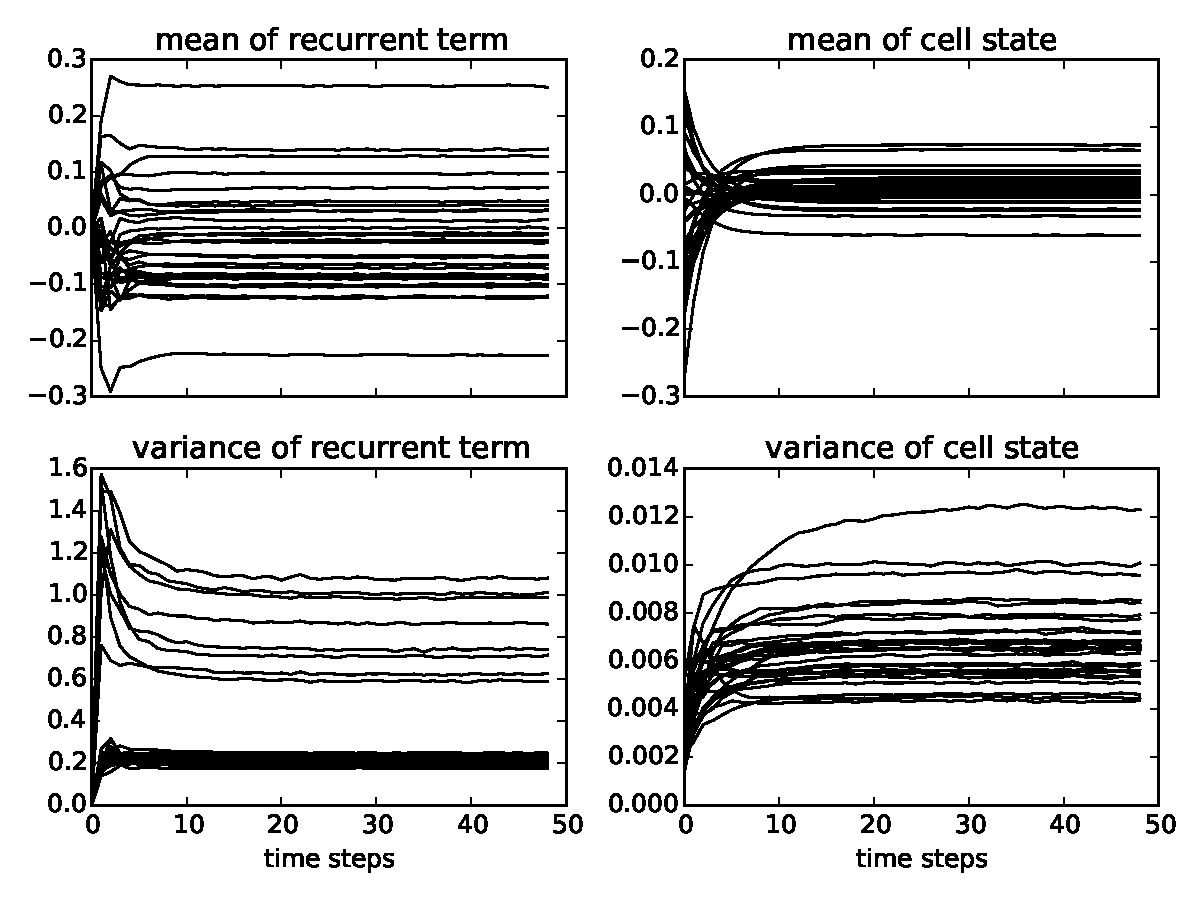
\includegraphics[width=0.8\textwidth]{figures/popstat_stationarity.pdf}
\caption{Convergence of population statistics to stationary distributions on the Penn Treebank task. Only a random subset of population statistics is shown.}
\label{fig:popstat_stationarity}
\end{figure}

During training we estimate the statistics across the minibatch, independently for each timestep.
At test time we use estimates obtained by averaging the minibatch estimates over the training set.

It would seem natural to share the statistics that are used for normalization across time,
just as recurrent neural networks share their parameters over time.
However, figure~\ref{fig:popstat_stationarity} shows that although the activations do converge to a stationary distribution,
their statistics during the initial transient differ significantly.
We have found empirically that simply averaging statistics over time severely degrades performance.
Instead, we recommend using separate statistics for each timestep.

Generalizing the model to sequences longer than those seen during training
is straightforward thanks to the rapid convergence of the activations
to their steady-state distributions (cf. Figure~\ref{fig:popstat_stationarity}).
For our experiments we estimate the population statistics separately for each timestep $1, \ldots, T_{max}$ where $T_{max}$ is the length of the longest training sequence.
When at test time we need to generalize beyond $T_{max}$, we use the population statistic of time $T_{max}$ for all time steps following it.

%% [there is an annoying little detail here: there may be only a single example with length T, and so the population statistic is highly unreliable. in this case i would take an earlier population statistic instead, the exact choice determined by validation. how do we explain this concisely?]
%% [additionally, we haven't actually dealt with variable-length training sequences yet. this is another technicality that's easily hacked around but people will want to know i guess.]


\section{On the Importance of Pre-Activation Variances}

\begin{figure}
  \center%
  \subfigure[
Gradient flow through a batch-normalized $\tanh$ RNN as a function of $\gamma$.
High variance causes gradient vanishing.
]{%
    \label{fig:rnn_grad_prop}
    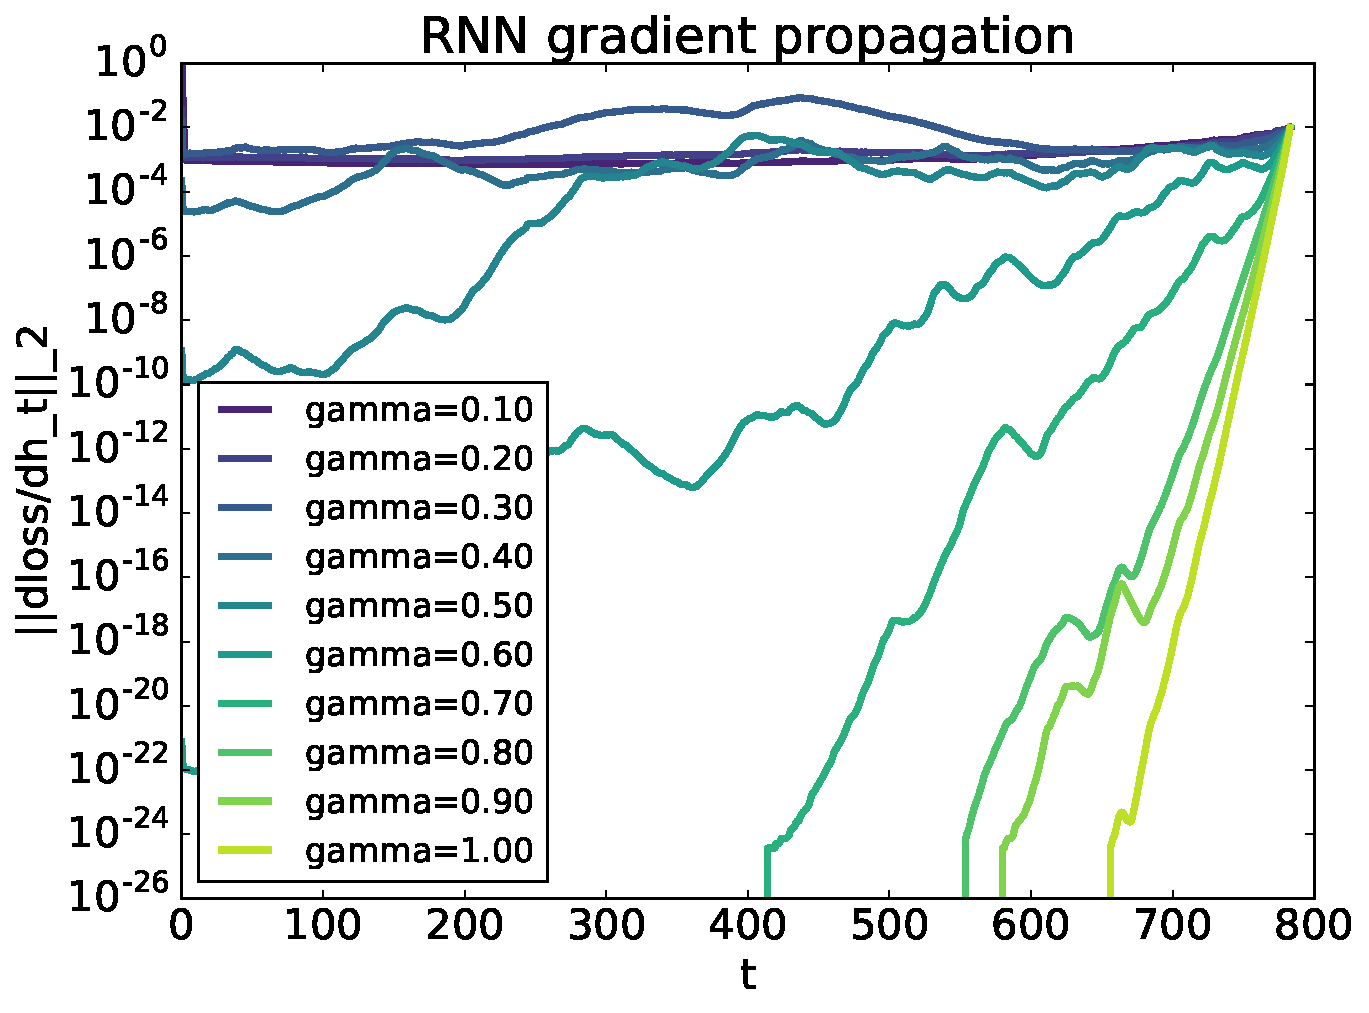
\includegraphics[width=.45\textwidth]{figures/rnn_grad_prop.pdf}
  }%
  \hspace{2mm}%
  \subfigure[
Empirical expected derivative of $\tanh$ nonlinearity as a function of input variance.
High variance causes saturation, which decreases the expected derivative.
]{%
    \label{fig:tanh_grad}
    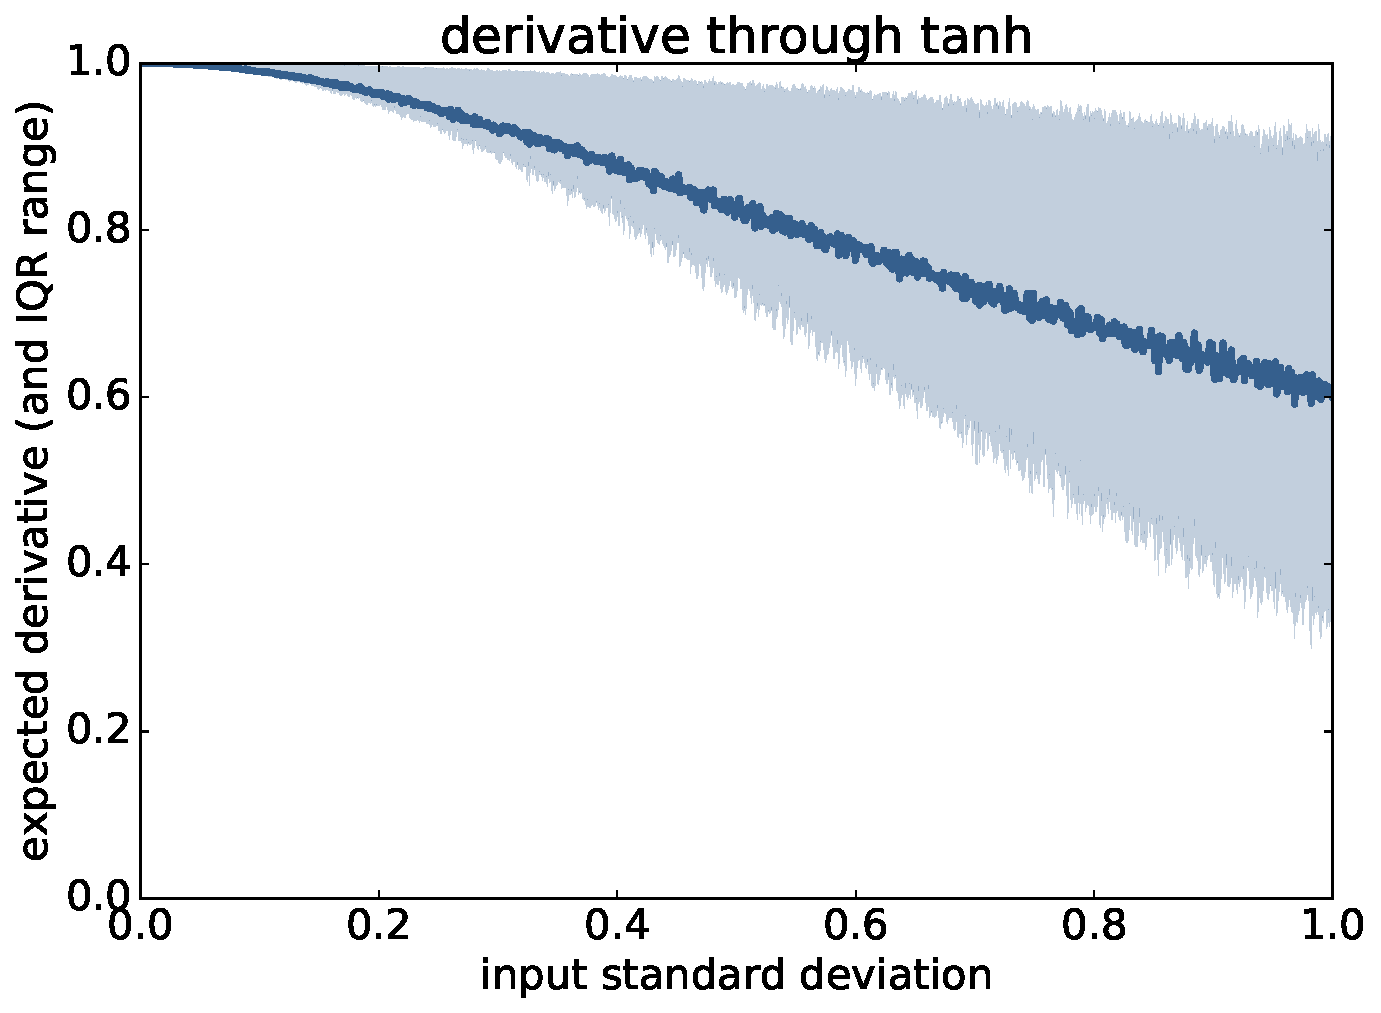
\includegraphics[width=.45\textwidth]{figures/tanh_grad.pdf}
  }
  \caption{
Influence of pre-activation variance on gradient propagation.
}
  \label{figure:DCNtradeoff}
\end{figure}

Although batch normalization allows for easy control of the pre-activation variance through the $\gamma$ parameters,
common practice is to normalize to unit variance.
We suspect that the previous difficulties with recurrent batch normalization reported in the literature~\cite{cesar,baidu}
are largely due to improper initialization of the batch normalization parameters, and $\gamma$ in particular.
In this section we demonstrate the impact of $\gamma$ on gradient flow.

In Figure~\ref{fig:rnn_grad_prop} we show how the pre-activation variance impacts gradient propagation in a simple RNN on the sequential MNIST task described in Section~\ref{sec:seqmnist}.
Since backpropagation operates in reverse, the plot is best read from right to left.
The quantity plotted is the norm of the gradient of the loss with respect to the hidden states.
For large values of $\gamma$, the norm quickly goes to zero as gradient is propagated back in time.
For small values of $\gamma$ the norm is nearly constant.

Figure~\ref{fig:tanh_grad} shows empirically how the expected derivative of the $\tanh$ nonlinearity changes with the variance of the argument.
When the input variance is low, the input tends to be close to the origin where the derivative is close to 1.
As the variance increases, the expected derivative decreases as the input is more likely to be in the saturation regime.
At unit variance, the expected derivative is much smaller than 1.
We conjecture that this is what causes the gradient to vanish.

% include lstm grad plot and speculate...?

\section{Experiments}
\label{sec:experiments}

\subsection{Sequential MNIST}
\label{sec:seqmnist}

\begin{figure}
\center
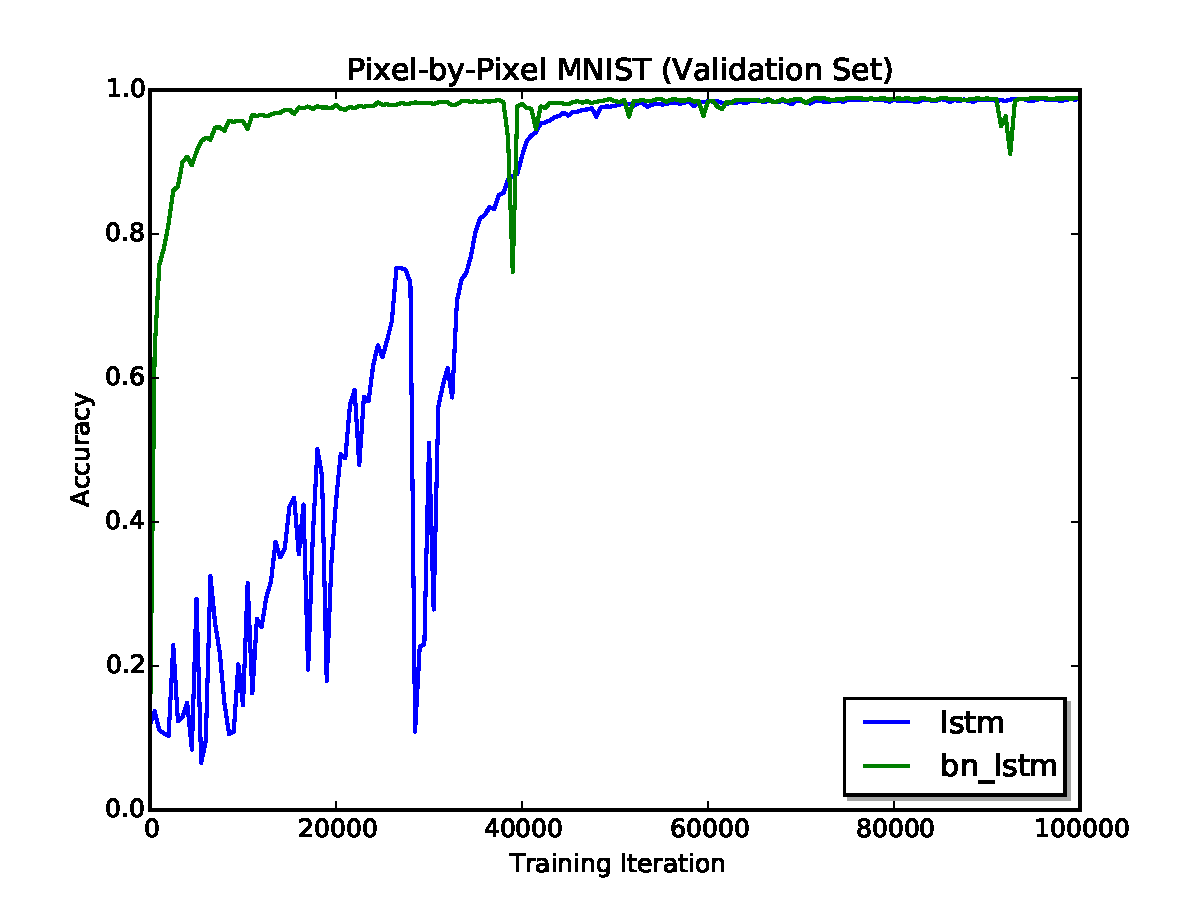
\includegraphics[width=6.7cm]{figures/unpermuted_valid.pdf}
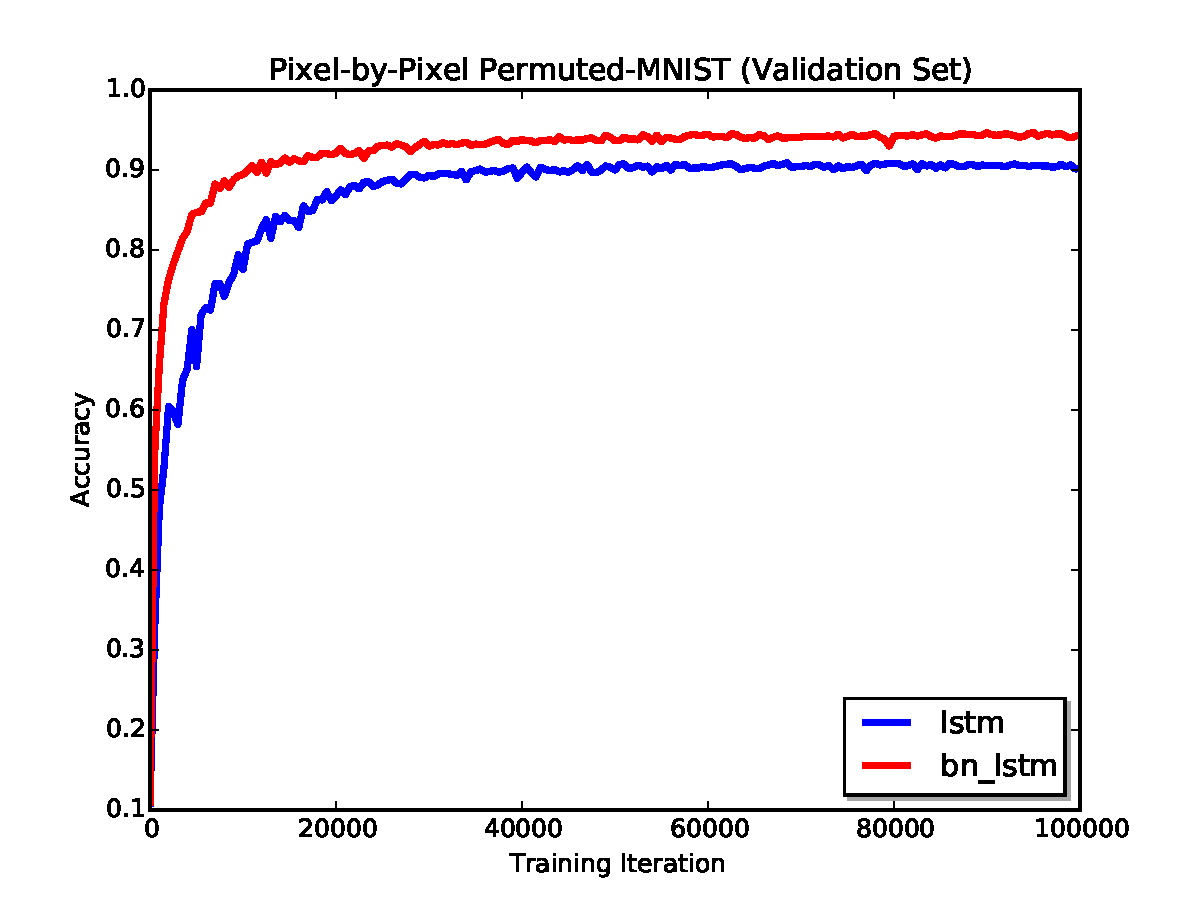
\includegraphics[width=6.7cm]{figures/permuted_valid.pdf}
\caption{Accuracy on the validation set for the pixel by pixel MNIST classification tasks. The batch-normalized LSTM is able to converge faster relatively to a baseline LSTM.
  Batch-normalized  LSTM also shows some improve generalization on the permuted sequential MNIST that require to preserve long-term memory information.}
\label{fig:seqmnist_valid}
\end{figure}


We evaluate recurrent batch normalization on a modified version of the MNIST dataset, suggested by~\cite{le2015simple}.
Recurrent models are fed MNIST pixels sequentially and have to output at the end of the sequence the corresponding MNIST label.
We consider two sequentall tasks, MNIST and $p$-(ermuted)MNIST, with different pixel ordering, MNIST considers the pixels from left to right, while $p$-MNIST uses and random ordering of the pixels.
As model, we consider a LSTM using $100$ hidden units. A softmax classifier
is applied on the final hidden representation.
LSTM relies on orthogonal initialization for the weight matrix, except for the hidden-to-hidden weight matrix that used identity initiliazation, as we observe better generalization performance with this
initiliaziation for this tasks.
The model is trained using RMSProp~\cite{rmsprop} with learning rate of $10^{-3}$ and a decay rate of $0.9$. We apply gradient clipping at 1 to avoid exploding gradients.

The initial states $\vect{h}_0$ are independent of the input and thus have zero variance.
This problem is exacerbated in unnatural data such as MNIST and various pathological tasks, where some features are constant across the data.
In the sequential MNIST task in particular, the variance is typically exactly zero for the first hundred or so time steps, as the upper pixels are almost always black.
Normalizing these zero-variance activations involves division by a very small number at many timesteps, which causes the gradient to explode.
We work around this by injecting noise into the initial hidden states.
Although the normalization amplifies the noise to signal level, we find that it does not hurt performance compared to data-dependent ways of initializing the hidden states.
%[but is that an artifact of classification at the end?]


\begin{table}
\center
\small
\begin{tabular}{c|c|c}
  & UnPermuted & Permuted\\
  \hline
  TANH-RNN~\cite{le2015simple} & 35.0 & 35.0\\
  $i$RNN~\cite{le2015simple} & 97.0 & 82.0\\
  $u$RNN~\cite{urnn} & 95.1 & 91.4\\
  $s$TANH-RNN~\cite{zhang2016architectural} & 98.1 & 94.0\\
  \hline
  LSTM & 98.9 & 90.2\\
  BN-LSTM & \textbf{99.0} & \textbf{95.4}\\
\end{tabular}
\caption{Accuracy obtained on the test set for the pixel by pixel MNIST classification tasks}
\label{tab:seqmnist_test}

\end{table}



Figure~\ref{fig:seqmnist_valid} reports the validation accuracy throught the training of both LSTM and batch-normalized LSTM (BN-LSTM). Figure~\ref{fig:seqmnist_valid} clearly shows recurrent batch normalization eases the model optimization, as batch-normalized LSTM converges faster than the baseline LSTM on both tasks.
In addition, we observe that batch-normalized LSTM obtain a significant generalization improvement on $p$-MNIST. It has been highlighted in~\cite{urnn}
that $p$-MNIST creates many longer term dependencies across pixels than in
the original pixel ordering, where a lot of structure is local. A recurrent network therefore needs to characterize dependencies across varying time scales in order to solve this tasks. Results show by using recurrent batch-normalization, we can learn a LSTM that better characterize those long-term dependencies.



Table~\ref{tab:seqmnist_test} reports the test set accuracy of the early stop model for the LSTM and BN-LSTM models using the population statistics. Recurrent batch normalization leds to better test score, especially for $p$-MNIST  where models have to leverage long-term temporal depencies. In addition, Table~\ref{tab:seqmnist_test} shows that our batch normalized LSTM achieves state-of-art on both MNIST and $p$-MNIST.

\subsection{Character-level Penn Treebank}

We evaluate our model on the task of character-level language modeling on the Penn Treebank corpus~\cite{penntreebank}.
We follow the setup of~\cite{krueger}, dividing the training set into nonoverlapping subsequences of length 50.
Our baseline is an LSTM with 1000 units.
We use stochastic gradient descent on minibatches of size 100,
with gradient clipping at 1.0 and step rule determined by RMSProp~\cite{rmsprop}
with learning rate 0.1 and momentum 0.9.
We use orthogonal initialization for all weight matrices.
The setup for the batch-normalized LSTM is the same in all respects except for the introduction of batch normalization.

%TODO move the repeat-population-statistics technicalities here

We were unable to reproduce the baseline reported in~\cite{krueger} and so are unable to compare directly to their results.
However, we show that batch normalizing our best baseline enables it to train faster and generalize better.

%\begin{figure}
%\center
%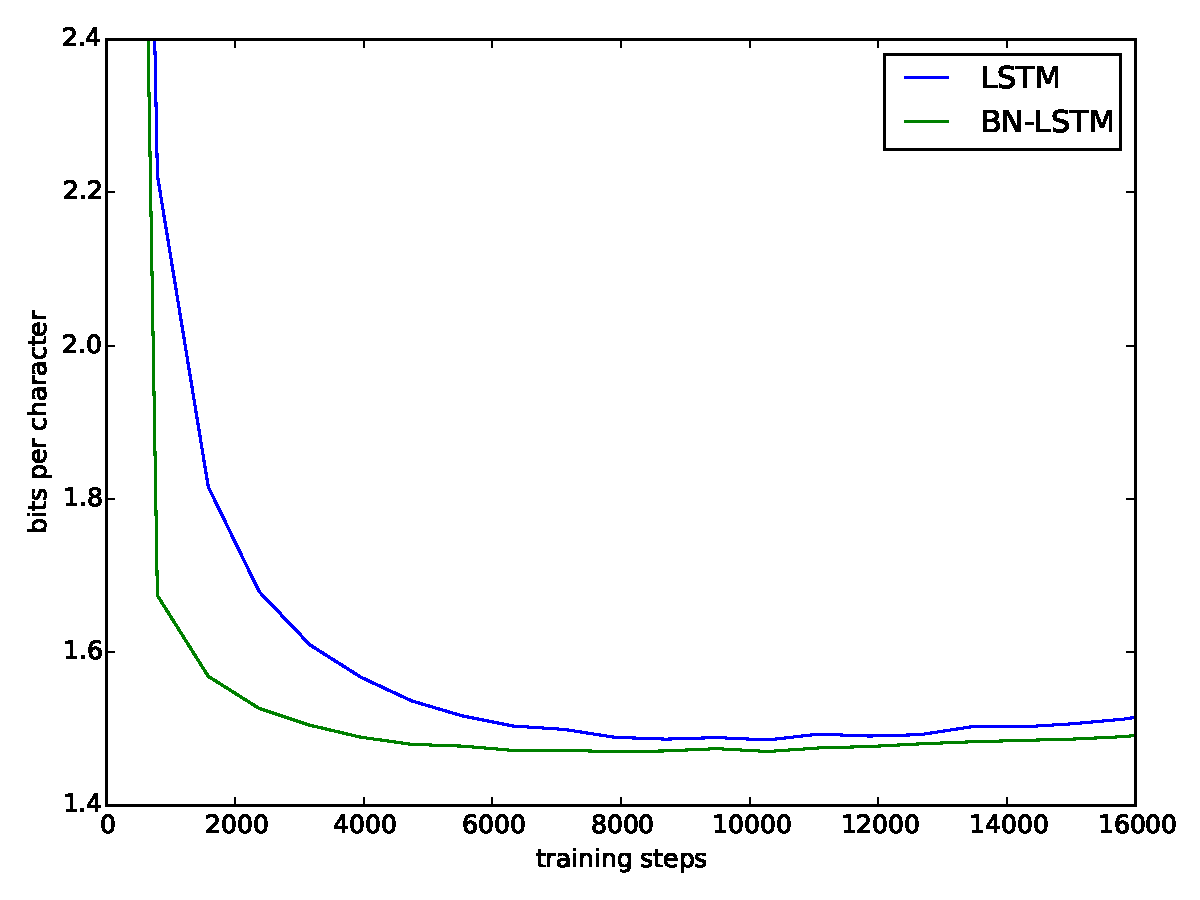
\includegraphics[width=7cm]{figures/ptb_valid.pdf}
%\caption{Bits-per-character on the validation set for Penn Treebank during training.}
%\label{fig:ptb_valid}
%\end{figure}

\begin{table}
\center
\begin{tabular}{c|c}
  & Penn Treebank \\
  \hline
  LSTM~\cite{graves2013generating} & 1.26
\footnote{Our performance does not directly compare against~\cite{graves2013generating} as they used a different dataset split.}
\\
  LSTM with norm stabilizer~\cite{krueger} & 1.39 \\
  \hline
  LSTM & NaN \\
  BN-LSTM & \textbf{NaN} \\
\end{tabular}
\caption{Bits-per-character on the Penn Treebank test string.}
\label{tab:ptb_test}
\end{table}

Table~\ref{tab:ptb_test} reports our performance in bits-per-character on the Penn Treebank test string.

\subsection{text8}

We evaluate our model on a second character-level language modeling task on the text8 dataset
\footnote{\url{http://mattmahoney.net/dc/textdata}}.
This dataset is derived from Wikipedia and consists of a string of 100M characters including only alphabetical characters and spaces.
We follow previous authors~\cite{mikolov2012subword,zhang2016architectural} and use the first 90M characters for training, the next 5M for validation and the final 5M characters for testing.
We train on nonoverlapping sequences of length 180.

\begin{table}
\center
\begin{tabular}{c|c}
  & text8 \\
  \hline
  $td$-LSTM~\cite{zhang2016architectural} & 1.63 \\
  HF-MRNN~\cite{mikolov2012subword} & 1.54 \\
  skipping RNN~\cite{pachitariu2013regularization} & 1.48 \\
  \hline
  LSTM & NaN \\
  BN-LSTM & \textbf{NaN} \\
\end{tabular}
\caption{Bits-per-character on the text8 test string.}
\label{tab:text8_test}
\end{table}

Table~\ref{tab:text8_test} reports our performance in bits-per-character on the text8 test string.

\subsection{TIMIT}

[do we include this? I'm not opposed to it but not sure what to say]

\subsection{Teaching Machines to Read and Comprehend}

To demonstrate the generality and practical applicability of our
re-parameterization, we take an implementation
\footnote{The code can be found at \url{https://github.com/caglar/Attentive_reader}}
of the Attentive Reader model~\cite{attentivereader} and simply replace the LSTM with our
BN-LSTM.
Additionally we try a variant where we also introduce batch
normalization into the attention computations, normalizing each term
going into the tanh nonlinearities.
Without any tweaking, we gain dramatic acceleration of training (Figure~\ref{fig:attr_valid}).

[Caglar will write a blurb on how the subset of data is selected]

\begin{figure}
\center
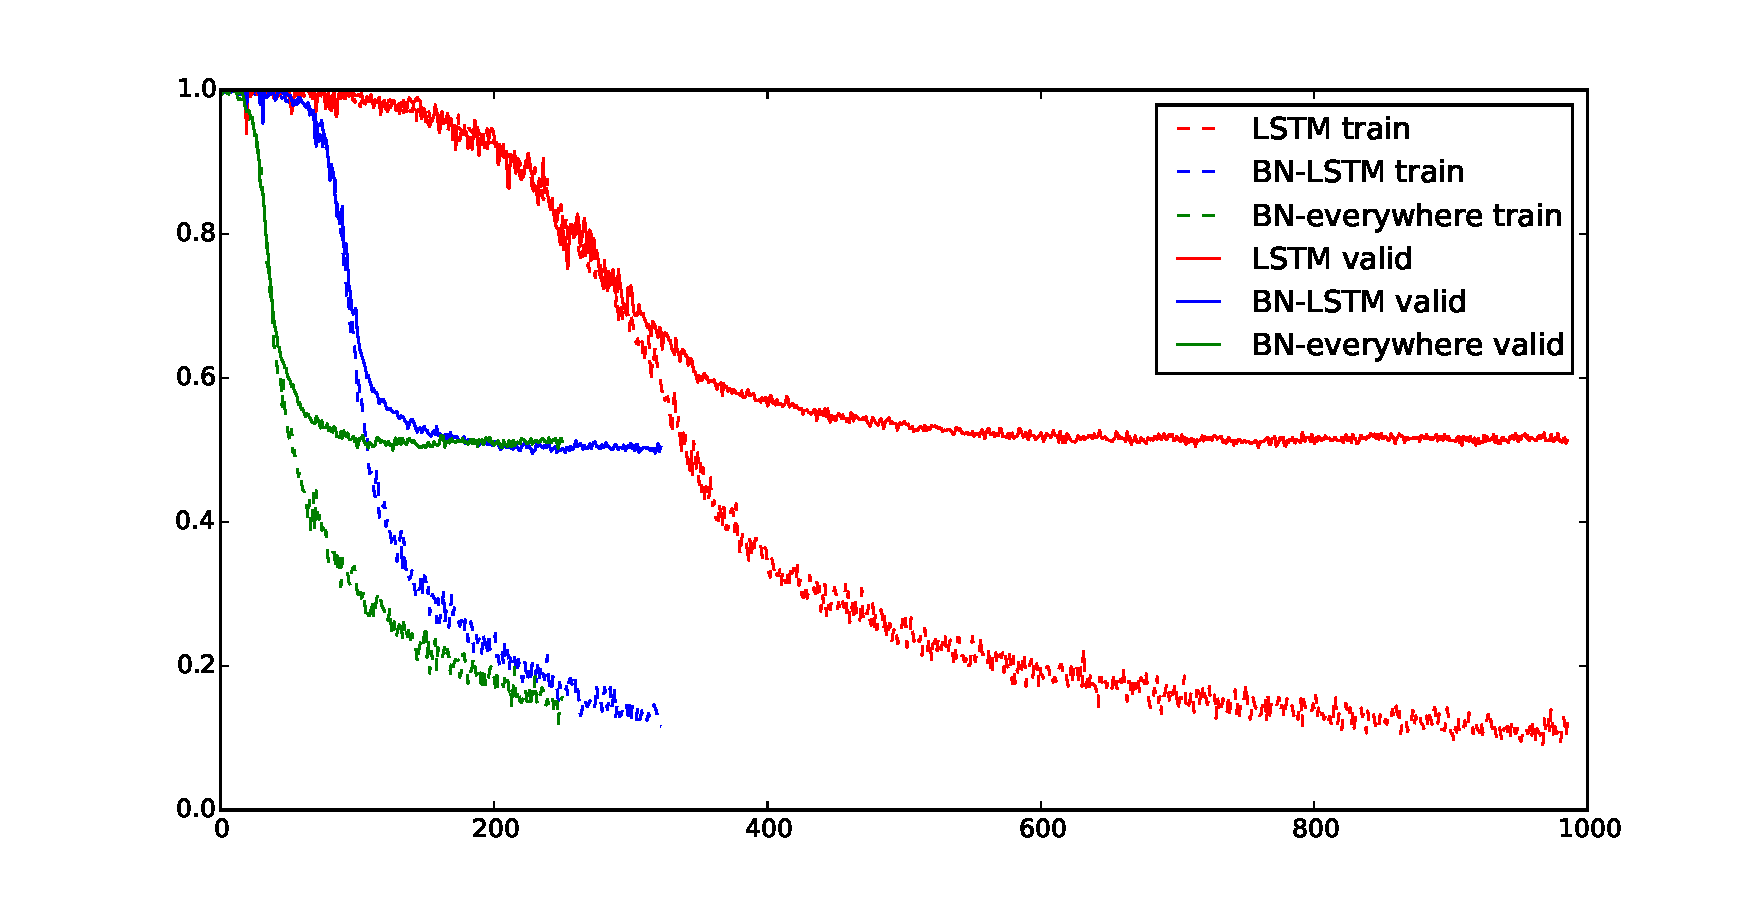
\includegraphics[width=0.8\textwidth]{figures/attr_valid.pdf}
\caption{
Accuracy on the validation set for the Attentive Reader models on a variant of the CNN QA task~\cite{attentivereader}.
BN-LSTM converges much faster than the baseline LSTM.
Applying batch normalization in the attention computations as well (``BN-everywhere'') converges faster yet.
}
\label{fig:attr_valid}
\end{figure}

\section{Conclusion}

\section*{Acknowledgements}

Experiments were conducted using the Theano~\cite{theano1}~\cite{theano2} and Blocks and Fuel~\cite{blocks} libraries.
[how to acknowledge use of cluster?]
We thank Çağlar Gülçehre for sharing his implementation of Attentive Reader and for helping us with experiments,
and David Krueger, Ishmael Belghazi and Saizheng Zhang for helpful discussions.

\bibliography{index}
\bibliographystyle{nips2015}

\end{document}
